% !TEX program = xelatex
\documentclass{misisarticle}
\usepackage{mathtools}
\usepackage{balance}
\urlstyle{same}
\addto\captionsrussian{\renewcommand{\refname}{ЛИТЕРАТУРА}}
\grnti{}
\asjc{}
\oecd{}
\title{Достижимость ограничения пересмотра прогноза}
\misisauthor{Н.~О.~Карасев\footnotemark[1]}{Университет МИСИС}{Москва, Россия}{karasev.no@phystech.edu}
\hypersetup{
 pdftitle={Достижимость ограничения пересмотра прогноза},
 pdfauthor={Карасев Никита Олегович},
 pdfsubject={Многошаговое прогнозирование временных рядов},
 pdfkeywords={временные ряды, комбинация прогнозов, пересмотр прогноза},
 pdfcreator={}
}
\patchcmd{\maketitle}{Аннотация — }{Аннотация: }{}{}
\patchcmd{\maketitle}{Ключевые слова — }{Ключевые слова: }{}{}
\setabstract{При последовательном прогнозировании меняется оценка одной и той же будущей величины. Рассмотрена смесь двух моделей с общим весом на весь горизонт. Для фиксированного прошлого выпуска получены минимальный достижимый пересмотр и точное условие выполнимости заданного ограничения. Условие позволяет отличить соблюдение ограничения от выбора наименее изменчивого прогноза при недостижимом допуске. Проверка проведена на одиннадцати часовых рядах с моделями DLinear и PatchTST. Все восемь конечных допусков, выбранных по валидации на основном горизонте, оказались невыполнимыми во всех тестовых выпусках. Снижение пересмотра в этих случаях объясняется минимизирующей ветвью правила и не означает выполнения ограничения.}
\setkeywords{временные ряды, комбинация прогнозов, адаптивный вес, пересмотр прогноза, достижимость}
\begin{document}
\maketitle
\footnotetext[1]{Научный руководитель: Филимонов Андрей Викторович.}

\section{Введение}

Диспетчер, который каждый час уточняет план энергопотребления на следующие четверо суток, получает несколько оценок для одного будущего часа. Даже точный в среднем прогноз может заметно меняться между выпусками. Поэтому ошибка относительно наблюдений и размер пересмотра отвечают на разные вопросы: первая характеризует точность, второй показывает, насколько сильно приходится обновлять уже составленный план.

Комбинирование моделей давно используется для повышения надежности прогноза~\cite{bates1969,wang2023}. Пересмотр можно учитывать при обучении нейронной сети или при обработке ее выходов~\cite{vanbelle2023,godahewa2025}. Здесь исследуется более узкий механизм: изменение одного веса между двумя готовыми прогнозами. Его вычислительная простота привлекательна, но сама по себе не означает, что любой заданный предел пересмотра выполним.

Цель работы состоит в проверке достижимости такого предела. Для каждого выпуска сначала определяется наименьшее возможное изменение в классе смесей, затем выбирается допустимый вес. Если ограничение невыполнимо, этот факт сохраняется в результатах, даже когда пересмотр удается уменьшить.

\section{Постановка задачи и условие достижимости}

В момент $t$ известны наблюдения $y_0,\ldots,y_t$. Две модели формируют векторы $a_t,b_t\in\mathbb R^H$, $H\geq2$: координата $h$ относится к моменту $t+h$. Их смесь имеет вид
\begin{equation}
 p_t(h)=b_t(h)+w_t\bigl(a_t(h)-b_t(h)\bigr),
 \quad w_t\in[0,1].
 \label{eq:mixture}
\end{equation}
Общий вес задает доверие к целой прогнозной траектории. Последовательные выпуски сравниваются на совпадающих будущих датах. При $m=H-1$ среднеквадратический пересмотр равен
\begin{equation}
 R_t=\sqrt{\frac1m\sum_{h=1}^{m}
      \bigl[p_t(h)-p_{t-1}(h+1)\bigr]^2}.
 \label{eq:revision}
\end{equation}
Новая последняя цель в это сравнение не входит. Величина $R_t$ вычисляется сразу при выпуске прогноза: будущие наблюдения для нее не нужны.

Пусть $\rho\geq0$ задает допустимый пересмотр. Даже неизменный вес не гарантирует $R_t\leq\rho$, поскольку обе базовые модели могут одновременно изменить свои прогнозы. Например, новые погодные данные сдвигают обе оценки температуры в одну сторону; замораживание веса этот сдвиг не устраняет.

Для фиксированного предыдущего выпуска введем векторы
\begin{equation}
 \begin{aligned}
 q_h&=p_{t-1}(h+1),\qquad d_h=a_t(h)-b_t(h),\\
 e_h&=b_t(h)-q_h,\qquad h=1,\ldots,m.
 \end{aligned}
 \label{eq:vectors}
\end{equation}
Далее $\langle x,z\rangle_m=m^{-1}\sum_hx_hz_h$ и
$\|x\|_m=\sqrt{\langle x,x\rangle_m}$. Зависимость пересмотра от текущего веса является квадратичной:
\begin{equation}
 \begin{aligned}
 R^2(w)&=\|e+wd\|_m^2=Aw^2+2Cw+D,\\
 A&=\langle d,d\rangle_m,\quad
 C=\langle d,e\rangle_m,\quad D=\langle e,e\rangle_m.
 \end{aligned}
 \label{eq:quadratic}
\end{equation}

\textbf{Утверждение.} Если $A>0$, минимальный достижимый пересмотр определяется выражениями
\begin{equation}
 w_*=\min\{1,\max\{0,-C/A\}\},\qquad
 F_t=\|e+w_*d\|_m.
 \label{eq:floor}
\end{equation}
Ограничение $R_t\leq\rho$ выполнимо тогда и только тогда, когда $F_t\leq\rho$. При выполнении этого условия допустимые веса образуют интервал
\begin{equation}
 \begin{aligned}
 I_t&=[0,1]\cap[w_-,w_+],\\
 w_\pm&=\frac{-C\pm\sqrt{C^2+A(\rho^2-D)}}{A}.
 \end{aligned}
 \label{eq:interval}
\end{equation}

\textit{Доказательство.} При $A>0$ функция~\eqref{eq:quadratic} строго выпукла, ее вершина находится в точке $-C/A$. Минимум на отрезке достигается в проекции вершины на $[0,1]$. Подуровневое множество непусто ровно при $\rho\geq F_t$; решение квадратного неравенства дает~\eqref{eq:interval}. Это частный случай стандартной задачи выпуклой оптимизации~\cite{boyd2004}.

При $A=0$ модели совпадают на общих целях. Тогда вес не влияет на пересмотр: $F_t=\sqrt D$.

Пусть $u_t\in[0,1]$ обозначает желаемый вес без прямого ограничения пересмотра, а $p_t^u$ смесь~\eqref{eq:mixture} при $w_t=u_t$. Рассматриваемое правило DirectRMS выбирает
\begin{equation}
 w_t=
 \begin{cases}
 \Pi_{I_t}(u_t),& F_t\leq\rho,\ A>0,\\
 u_t,& F_t\leq\rho,\ A=0,\\
 w_*,& F_t>\rho,\ A>0,\\
 u_t,& F_t>\rho,\ A=0,
 \end{cases}
 \label{eq:rule}
\end{equation}
где $\Pi_I$ означает проекцию на интервал. При невыполнимом ограничении правило минимизирует пересмотр, но не объявляет допуск соблюденным. Для каждого выпуска выполняется
\begin{equation}
 R_t\leq\max\{\rho,F_t\}.
 \label{eq:guarantee}
\end{equation}
Вычисление коэффициентов требует $O(H)$ операций.

\begin{figure*}[t]
 \centering
 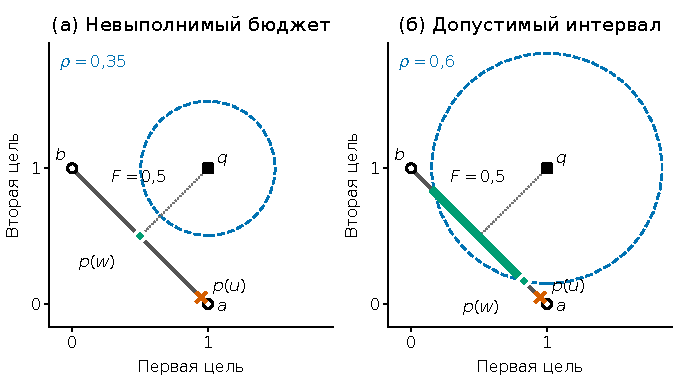
\includegraphics[width=0.76\textwidth]{figures/feasibility_geometry.pdf}
 \caption{Геометрический пример для двух общих целей:
 $a=(1,0)$, $b=(0,1)$, $q=(1,1)$, желаемый вес $u=0{,}95$.
 Отрезок задает доступные смеси, штриховая окружность соответствует RMS-допуску.
 Минимум $F=0{,}5$ достигается при $w_*=0{,}5$.
 При $\rho=0{,}35$ допустимых весов нет; при $\rho=0{,}6$ они образуют выделенный участок.
 Пример иллюстрирует формулу и не является измерением на данных.}
 \label{fig:geometry}
\end{figure*}

Граница $F_t$ относится к конкретному прошлому $q$. Если на предыдущем шаге использовать другой вес, изменятся следующий минимум и множество допустимых решений. Поэтому~\eqref{eq:floor} не является глобальным минимумом пересмотров за весь период. Геометрический смысл локального условия показан на рис.~\ref{fig:geometry}.

\section{Данные и вычислительный протокол}

Проверка использует часовые данные двух открытых источников. На станции WS Beutenberg Института биогеохимии Общества Макса Планка выбраны температура, давление и скорость ветра~\cite{weather}. В ElectricityLoadDiagrams20112014 из UCI рассматриваются восемь потребителей MT002-MT009~\cite{electricity}. Погодные наблюдения агрегируются из десятиминутных, потребление из пятнадцатиминутных значений. Одиннадцать рядов относятся к двум предметным источникам и не считаются независимыми областями применения.

Для погоды обучение проводится на 2018-2019 годах, валидация на 2020-м, тест на 2021-2022 годах. Для потребления используются соответственно 2012, 2013 и 2014 годы. Среднее и стандартное отклонение определяются только на обучающей части. Пропуски входной истории заполняются последним доступным значением; для оценки ошибки используются лишь полностью наблюдавшиеся целевые горизонты.

Взяты официальные реализации DLinear~\cite{dlinearcode} и supervised PatchTST~\cite{nie2023}. История содержит 336 часов, горизонт $H=96$ часов. Для каждой модели и ряда выполнены пять повторов с seed 11, 22, 33, 44 и 55.

DLinear использует окно разложения 25. PatchTST имеет три слоя, четыре головы, скрытую размерность 16, размер внутреннего слоя 128, длину патча 16 и шаг 8; dropout равен $0{,}3$, RevIN включен без обучаемого аффинного преобразования. Использованы Adam, batch 128 и не более 200 эпох с остановкой после 20 эпох без улучшения валидационной MSE. Шаг обучения выбирался на валидации из $10^{-4}$, $3\cdot10^{-4}$ и $10^{-3}$ на seed 11, затем переносился на остальные повторы. Здесь сравниваются готовые конфигурации в целом; из их разности нельзя выделить эффект механизма attention.

Желаемый вес Adaptive определяется по средним ошибкам экспертов $\bar\ell_a,\bar\ell_b$, где ошибка выпуска есть MSE полного наблюдавшегося горизонта:
\begin{equation}
 u_t=\left(1+\exp\{(\bar\ell_a-\bar\ell_b)/\tau\}\right)^{-1}.
 \label{eq:adaptive}
\end{equation}
Ошибка выпуска $r$ доступна только при $r+H\leq t$. Усреднение ведется по последним $K$ доступным ошибкам; до накопления очереди $u_t=1/2$. Параметры $K\in\{24,72,168,336\}$ и $\tau\in\{0{,}01;0{,}05;0{,}1;0{,}5;1\}$ выбираются по средней валидационной MSE пяти повторов. При равенстве предпочтение отдается большим $K$, затем $\tau$.

Помимо Adaptive используются постоянная смесь Fixed с весом, минимизирующим валидационную MSE отдельно для каждого seed, и интерполяция выпусков FI. Для общих целей последняя задается формулой
\begin{equation}
 p_t^{\rm FI}(h)=
 \gamma p_t^{u}(h)+(1-\gamma)p_{t-1}^{\rm FI}(h+1),
 \label{eq:fi}
\end{equation}
а новая последняя координата берется из $p_t^u$. Коэффициент $\gamma$ выбирается из $0$; $0{,}1$; $0{,}25$; $0{,}5$; $0{,}75$; $0{,}9$; $1$.

Для DirectRMS проверяется сетка $\rho$: $0$; $0{,}001$; $0{,}003$; $0{,}01$; $0{,}03$; $0{,}1$; $0{,}3$; $1$; $3$; $\infty$. Для обоих стабилизирующих правил выбирается наименьший средний RMS среди настроек с валидационной MSE не более чем на 1\% выше MSE Adaptive. При равенстве используются меньшая MSE, затем более слабое вмешательство. Если подходящих настроек нет, применяется Adaptive. При $\rho=\infty$ прямое ограничение отключено.

Бюджет и пересмотр выражаются в обучающих стандартных отклонениях ряда, MSE в их квадратах. Состояние каждой политики непрерывно проходит границу валидации и теста; желаемые веса не получают еще неизвестных ошибок. Все сравниваемые правила используют один архив прогнозов экспертов. Тестовые данные не участвуют в настройке параметров.

\section{Результаты и обсуждение}

\begin{table*}[t]
 \caption{DirectRMS относительно Adaptive при $H=96$. Относительные разности рассчитаны по средним пяти повторов; отрицательное значение означает уменьшение метрики. Доля невыполнимости относится к собственной последовательности прошлых выпусков DirectRMS.}
 \label{tab:results}
 \centering
 \begin{tabular}{lrrrrr}
\toprule
Ряд & $\rho$ & Невыполнимость, \% & $\Delta{\rm MSE}$, \% & $\Delta{\rm RMS}$, \% & $\mathrm{RMS}_{\rm DirectRMS}/\mathrm{RMS}_{\rm FI}$\\
\midrule
MPI T & $0{,}003$ & $100$ & $+0{,}64$ & $-8{,}21$ & $1{,}44$\\
MPI p & $\infty$ & $-$ & $0{,}00$ & $0{,}00$ & $1{,}23$\\
MPI wv & $0{,}01$ & $100$ & $+0{,}26$ & $-4{,}14$ & $2{,}98$\\
MT002 & $0{,}01$ & $100$ & $+0{,}43$ & $-4{,}87$ & $3{,}74$\\
MT003 & $0{,}001$ & $100$ & $-23{,}52$ & $-35{,}73$ & $5{,}79$\\
MT004 & $0{,}01$ & $100$ & $-0{,}28$ & $-3{,}50$ & $9{,}30$\\
MT005 & $0{,}01$ & $100$ & $+0{,}17$ & $-2{,}73$ & $3{,}70$\\
MT006 & $0{,}01$ & $100$ & $+0{,}19$ & $-6{,}13$ & $3{,}90$\\
MT007 & $\infty$ & $-$ & $0{,}00$ & $0{,}00$ & $1{,}93$\\
MT008 & $0{,}01$ & $100$ & $-1{,}21$ & $-6{,}63$ & $3{,}92$\\
MT009 & $\infty$ & $-$ & $0{,}00$ & $0{,}00$ & $4{,}07$\\
\bottomrule
\end{tabular}

 \par\smallskip
 \parbox{0.95\textwidth}{\footnotesize
 MPI T, MPI p и MPI wv обозначают температуру, давление и скорость ветра.
 Прочерк означает отключенное ограничение: DirectRMS совпадает с Adaptive.
 Для любой метрики $M$ относительная разность равна
 $100(\overline M_{\rm DirectRMS}-\overline M_{\rm Adaptive})/
 \overline M_{\rm Adaptive}$.
 Последний столбец сравнивает средние RMS; значение больше единицы соответствует меньшему пересмотру у FI.}
\end{table*}

\begin{figure*}[t]
 \centering
 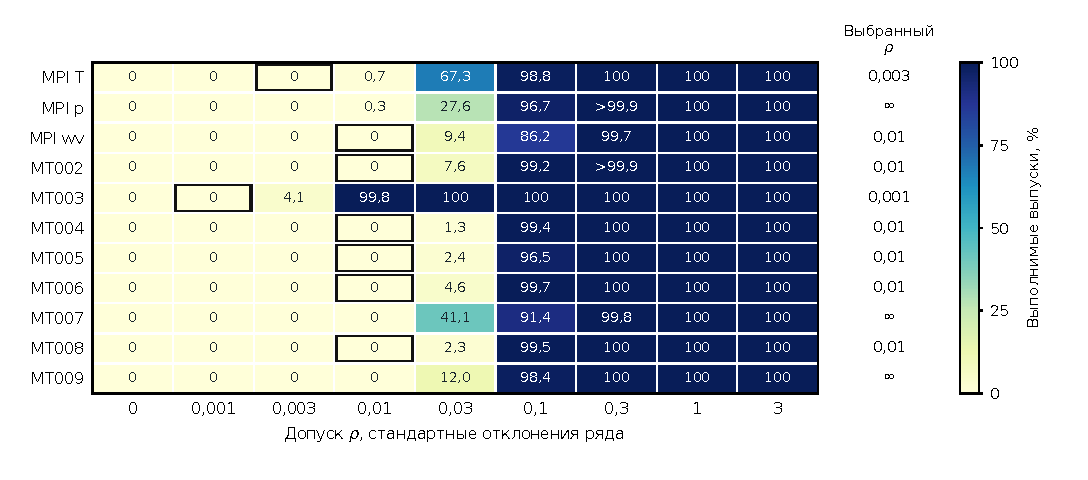
\includegraphics[width=0.96\textwidth]{figures/feasibility_budget.pdf}
 \caption{Доля выполнимых выпусков DirectRMS при $H=96$ на полной заранее заданной сетке конечных допусков.
 В ячейках указаны средние пяти повторов, в процентах.
 Рамками отмечены конечные настройки, выбранные по валидации; справа приведен выбранный допуск для каждого ряда.
 Значение $\infty$ означает отключенное ограничение.
 Каждый допуск использует собственную последовательность прошлых выпусков.}
 \label{fig:feasibility-budget}
\end{figure*}

На основном горизонте валидация выбрала восемь конечных бюджетов. Каждый из них оказался невыполнимым на всех тестовых выпусках во всех пяти повторах. В этих случаях DirectRMS совпал с правилом выбора локального минимума $w_*$. Для давления, MT007 и MT009 выбран бесконечный бюджет, поэтому эти три варианта совпадают с Adaptive (табл.~\ref{tab:results}).

Температурный ряд показывает, почему важно проверять само ограничение. При $\rho=0{,}003$ средний пересмотр равен $0{,}03072$: он меньше значения Adaptive $0{,}03347$, но примерно в десять раз выше заданного допуска. Снижение на 8,21\% нельзя описывать как выполнение ограничения. Оно получено благодаря переходу к минимизирующей ветви.

Точность и стабильность меняются неодинаково. Среди восьми конечных вариантов MSE относительно Adaptive уменьшается на трех рядах и увеличивается на пяти. На MT003 снижение MSE составляет 23,52\%, RMS 35,73\%. Однако относительно постоянной смеси Fixed разность MSE здесь равна лишь $-0{,}19\%$, а RMS $-3{,}57\%$. Большой эффект относительно Adaptive поэтому не означает такого же преимущества над простой постоянной комбинацией.

FI дает меньший средний RMS на всех одиннадцати рядах. Для температуры его RMS равен $0{,}02134$, тогда как MSE составляет $0{,}20427$ против $0{,}20423$ у DirectRMS. Эти близкие точечные ошибки не доказывают эквивалентности методов. Приведенные средние характеризуют наблюдавшиеся различия; статистическая значимость по ним не устанавливается.

Результат FI не противоречит условию достижимости. Интерполяция использует предыдущий выпуск и не ограничена отрезком между текущими прогнозами экспертов. Поэтому $F_t$ не является нижней границей ее пересмотра. Условие~\eqref{eq:floor} характеризует возможности выбранной смеси при данном прошлом, а не любых методов прогнозирования.

Полная заранее заданная сетка показывает, как меняется достижимость при других допусках (рис.~\ref{fig:feasibility-budget}). При $\rho=0{,}03$ средняя по пяти повторам доля выполнимых выпусков составляет от 1,29\% на MT004 до 100\% на MT003. При $\rho=0{,}1$ она превышает 86\% на каждом ряду; при $\rho=1$ ограничение соблюдается во всех выпусках всех пяти повторов. Это не новые настройки, выбранные по тесту, а описание всей зафиксированной сетки. Увеличение допуска облегчает его соблюдение, но само по себе не доказывает улучшения точности.

У каждого допуска своя история выпущенных прогнозов, а значит, и свои значения $F_t$. Поэтому матрица не является распределением одной неизменной границы. Она дополняет условие достижимости наблюдаемыми частотами для разных политик. Данные одной станции и восьми потребителей не позволяют переносить эти частоты на другие предметные области.

\balance
\section{Заключение}

Для смеси двух многошаговых прогнозов проверка ограничения пересмотра сводится к одномерной квадратичной задаче. Полученное условие отделяет допустимое управление весом от наименее изменчивого решения при недостижимом допуске. На рассмотренных рядах уменьшение пересмотра после выбора параметров часто обеспечивалось именно второй ветвью. Практический вывод состоит в том, что вместе с ошибкой и средним пересмотром нужно сообщать долю невыполнимых выпусков. Без нее более стабильный прогноз легко принять за выполнение ограничения, которое фактически не соблюдалось.

\begin{thebibliography}{9}
\bibitem{bates1969}
J.~M. Bates, C.~W.~J. Granger.
The Combination of Forecasts.
\textit{Journal of the Operational Research Society},
vol.~20, no.~4, pp.~451-468, 1969.
DOI: \url{https://doi.org/10.1057/jors.1969.103}.

\bibitem{wang2023}
X. Wang, R.~J. Hyndman, F. Li, Y. Kang.
Forecast combinations: An over 50-year review.
\textit{International Journal of Forecasting},
vol.~39, no.~4, pp.~1518-1547, 2023.
DOI: \url{https://doi.org/10.1016/j.ijforecast.2022.11.005}.

\bibitem{vanbelle2023}
J. Van Belle, R. Crevits, W. Verbeke.
Improving forecast stability using deep learning.
\textit{International Journal of Forecasting},
vol.~39, no.~3, pp.~1333-1350, 2023.
DOI: \url{https://doi.org/10.1016/j.ijforecast.2022.06.007}.

\bibitem{godahewa2025}
R. Godahewa et al.
On forecast stability.
\textit{International Journal of Forecasting},
vol.~41, no.~4, pp.~1539-1558, 2025.
DOI: \url{https://doi.org/10.1016/j.ijforecast.2025.01.006}.

\bibitem{boyd2004}
S. Boyd, L. Vandenberghe.
\textit{Convex Optimization}.
Cambridge University Press, 2004.
DOI: \url{https://doi.org/10.1017/CBO9780511804441}.

\bibitem{weather}
Max Planck Institute for Biogeochemistry.
Weather station WS Beutenberg.
\url{https://www.bgc-jena.mpg.de/wetter/weather_data.html}.

\bibitem{electricity}
UCI Machine Learning Repository.
ElectricityLoadDiagrams20112014.
\url{https://archive.ics.uci.edu/dataset/321/electricityloaddiagrams20112014}.

\bibitem{dlinearcode}
LTSF-Linear. Official implementation.
Version \texttt{0c113668a3b8}.
\url{https://github.com/cure-lab/LTSF-Linear}.

\bibitem{nie2023}
Y. Nie, N.~H. Nguyen, P. Sinthong, J. Kalagnanam.
A Time Series is Worth 64 Words:
Long-term Forecasting with Transformers.
\textit{International Conference on Learning Representations}, 2023.
\url{https://openreview.net/forum?id=Jbdc0vTOcol}.
\end{thebibliography}
\end{document}
